\chapter{Arbres d'expansió}

\index{arbre d'expansió}

Un \key{arbre d'expansió} (\emph{spanning tree}) d'un graf és un arbre
que conté tots els nodes del graf i algunes de les arestes. Com que és
un arbre, els arbres d'expansió són connexos, acíclics i existeix un
sol camí entre dos nodes qualsevol. Normalment hi ha diverses maneres
de construir un arbre d'expansió.

Per exemple, considereu el graf següent:
\begin{center}
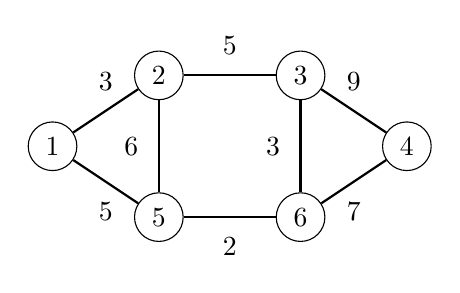
\begin{tikzpicture}[scale=0.9]
\node[draw, circle] (1) at (1.5,2) {$1$};
\node[draw, circle] (2) at (3,3) {$2$};
\node[draw, circle] (3) at (5,3) {$3$};
\node[draw, circle] (4) at (6.5,2) {$4$};
\node[draw, circle] (5) at (3,1) {$5$};
\node[draw, circle] (6) at (5,1) {$6$};
\path[draw,thick,-] (1) -- node[font=\small,label=above:3] {} (2);
\path[draw,thick,-] (2) -- node[font=\small,label=above:5] {} (3);
\path[draw,thick,-] (3) -- node[font=\small,label=above:9] {} (4);
\path[draw,thick,-] (1) -- node[font=\small,label=below:5] {} (5);
\path[draw,thick,-] (5) -- node[font=\small,label=below:2] {} (6);
\path[draw,thick,-] (6) -- node[font=\small,label=below:7] {} (4);
\path[draw,thick,-] (2) -- node[font=\small,label=left:6] {} (5);
\path[draw,thick,-] (3) -- node[font=\small,label=left:3] {} (6);
\end{tikzpicture}
\end{center}
Un possible arbre d'expansió és el següent:
\begin{center}
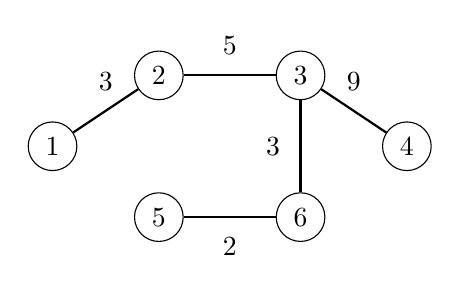
\begin{tikzpicture}[scale=0.9]
\node[draw, circle] (1) at (1.5,2) {$1$};
\node[draw, circle] (2) at (3,3) {$2$};
\node[draw, circle] (3) at (5,3) {$3$};
\node[draw, circle] (4) at (6.5,2) {$4$};
\node[draw, circle] (5) at (3,1) {$5$};
\node[draw, circle] (6) at (5,1) {$6$};
\path[draw,thick,-] (1) -- node[font=\small,label=above:3] {} (2);
\path[draw,thick,-] (2) -- node[font=\small,label=above:5] {} (3);
\path[draw,thick,-] (3) -- node[font=\small,label=above:9] {} (4);
\path[draw,thick,-] (5) -- node[font=\small,label=below:2] {} (6);
\path[draw,thick,-] (3) -- node[font=\small,label=left:3] {} (6);
\end{tikzpicture}
\end{center}


El pes d'un arbre d'expansió és la suma dels pesos de les seves
arestes. Per exemple, el pes de l'arbre d'expansió anterior és
$3+5+9+3+2=22$.

\index{arbre d'expansió mínim}

Un \key{arbre d'expansió mínim} és aquell que té pes mínim. En
l'exemple anterior, el pes mínim és 20, i aquest arbre es pot
construir com segueix:


\begin{center}
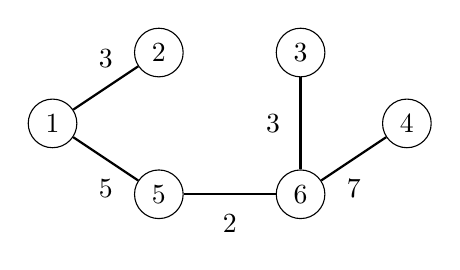
\begin{tikzpicture}[scale=0.9]
\node[draw, circle] (1) at (1.5,2) {$1$};
\node[draw, circle] (2) at (3,3) {$2$};
\node[draw, circle] (3) at (5,3) {$3$};
\node[draw, circle] (4) at (6.5,2) {$4$};
\node[draw, circle] (5) at (3,1) {$5$};
\node[draw, circle] (6) at (5,1) {$6$};

\path[draw,thick,-] (1) -- node[font=\small,label=above:3] {} (2);
\path[draw,thick,-] (1) -- node[font=\small,label=below:5] {} (5);
\path[draw,thick,-] (5) -- node[font=\small,label=below:2] {} (6);
\path[draw,thick,-] (6) -- node[font=\small,label=below:7] {} (4);
\path[draw,thick,-] (3) -- node[font=\small,label=left:3] {} (6);
\end{tikzpicture}
\end{center}


\index{arbre d'expansió màxim}

De la mateixa manera, un \key{arbre d'expansió màxim} és aquell que té
pes màxim. En l'exemple anterior és 32:

\begin{center}
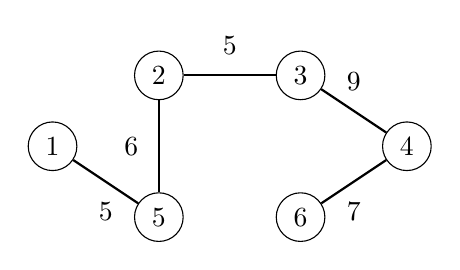
\begin{tikzpicture}[scale=0.9]
\node[draw, circle] (1) at (1.5,2) {$1$};
\node[draw, circle] (2) at (3,3) {$2$};
\node[draw, circle] (3) at (5,3) {$3$};
\node[draw, circle] (4) at (6.5,2) {$4$};
\node[draw, circle] (5) at (3,1) {$5$};
\node[draw, circle] (6) at (5,1) {$6$};
\path[draw,thick,-] (2) -- node[font=\small,label=above:5] {} (3);
\path[draw,thick,-] (3) -- node[font=\small,label=above:9] {} (4);
\path[draw,thick,-] (1) -- node[font=\small,label=below:5] {} (5);
\path[draw,thick,-] (6) -- node[font=\small,label=below:7] {} (4);
\path[draw,thick,-] (2) -- node[font=\small,label=left:6] {} (5);
\end{tikzpicture}
\end{center}


Tingueu en compte que un graf pot tenir diversos arbres d'expansió
mínims i màxims, de manera que els arbres no són únics.

Resulta que es poden fer servir diversos algorismes greedy per
construir arbres d'expansió mínim i màxim. En aquest capítol, discutim
dos algorismes que processen les arestes del graf ordenades segons els
seus pesos. Ens centrem en trobar arbres d'expansió mínim, però els
mateixos algorismes poden trobar arbres d'expansió màxim processant
les arestes en ordre invers.

\section{Algorisme de Kruskal}

\index{Algorisme de Kruskal}

En l'\key{algorisme de Kruskal}\footnote{L'algorisme va ser publicat
l'any 1956 per J. B. Kruskal \cite{kru56}.}, omplirem un arbre
d'expansió aresta a aresta. L'algorisme recorre totes les arestes
ordenades pels seus pesos, i afegeix l'aresta si no crea cap cicle amb
les arestes ja seleccionades.

L'algorisme manté les components connexes de l'arbre d'expansió que
estem omplint. Inicialment, cadascun dels $n$ nodes del graf pertany a
una component connexa distinta. Només afegim arestes quan unim dues
components distintes, ja que altrament tindríem un cicle. L'algorisme
acaba quan, després d'afegir $n-1$ arestes, tenim una sola component
connexa resultant. Quan això passa hem trobat un arbre d'expansió
mínim.

\subsubsection{Exemple}


\begin{samepage}
Let us consider how Kruskal's algorithm processes the
following graph:
\begin{center}
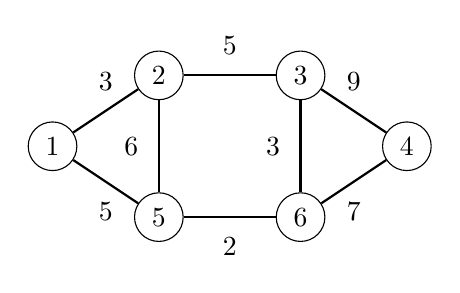
\begin{tikzpicture}[scale=0.9]
\node[draw, circle] (1) at (1.5,2) {$1$};
\node[draw, circle] (2) at (3,3) {$2$};
\node[draw, circle] (3) at (5,3) {$3$};
\node[draw, circle] (4) at (6.5,2) {$4$};
\node[draw, circle] (5) at (3,1) {$5$};
\node[draw, circle] (6) at (5,1) {$6$};
\path[draw,thick,-] (1) -- node[font=\small,label=above:3] {} (2);
\path[draw,thick,-] (2) -- node[font=\small,label=above:5] {} (3);
\path[draw,thick,-] (3) -- node[font=\small,label=above:9] {} (4);
\path[draw,thick,-] (1) -- node[font=\small,label=below:5] {} (5);
\path[draw,thick,-] (5) -- node[font=\small,label=below:2] {} (6);
\path[draw,thick,-] (6) -- node[font=\small,label=below:7] {} (4);
\path[draw,thick,-] (2) -- node[font=\small,label=left:6] {} (5);
\path[draw,thick,-] (3) -- node[font=\small,label=left:3] {} (6);
\end{tikzpicture}
\end{center}
\end{samepage}



\begin{samepage}
The first step of the algorithm is to sort the
edges in increasing order of their weights.
The result is the following list:

\begin{tabular}{ll}
\\
edge & weight \\
\hline
5--6 & 2 \\
1--2 & 3 \\
3--6 & 3 \\
1--5 & 5 \\
2--3 & 5 \\
2--5 & 6 \\
4--6 & 7 \\
3--4 & 9 \\
\\
\end{tabular}
\end{samepage}


Després d'això, l'algorisme recorre la llista i afegeix cada aresta a
l'arbre si aquesta uneix dues components separades.

Inicialment, cada node té la seva pròpia component connexa:


\begin{center}
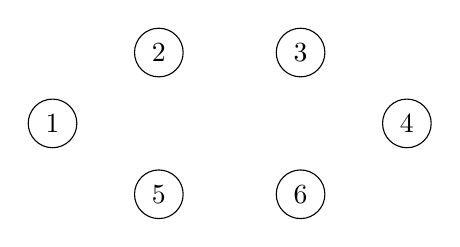
\begin{tikzpicture}[scale=0.9]
\node[draw, circle] (1) at (1.5,2) {$1$};
\node[draw, circle] (2) at (3,3) {$2$};
\node[draw, circle] (3) at (5,3) {$3$};
\node[draw, circle] (4) at (6.5,2) {$4$};
\node[draw, circle] (5) at (3,1) {$5$};
\node[draw, circle] (6) at (5,1) {$6$};
%\path[draw,thick,-] (1) -- node[font=\small,label=above:3] {} (2);
%\path[draw,thick,-] (2) -- node[font=\small,label=above:5] {} (3);
%\path[draw,thick,-] (3) -- node[font=\small,label=above:9] {} (4);
%\path[draw,thick,-] (1) -- node[font=\small,label=below:5] {} (5);
%\path[draw,thick,-] (5) -- node[font=\small,label=below:2] {} (6);
%\path[draw,thick,-] (6) -- node[font=\small,label=below:7] {} (4);
%\path[draw,thick,-] (2) -- node[font=\small,label=left:6] {} (5);
%\path[draw,thick,-] (3) -- node[font=\small,label=left:3] {} (6);
\end{tikzpicture}
\end{center}
La primera aresta que s'afegeix a l'arbre és la aresta 5--6 que crea
la component $\{5,6\}$ resultant d'unir les components $\{5\}$ i $\{6\}$:


\begin{center}
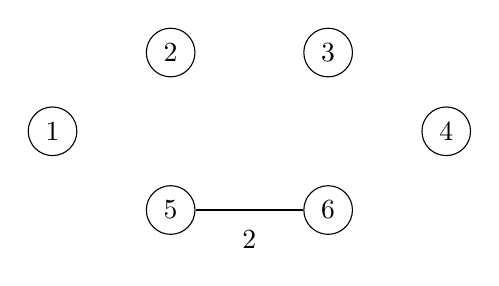
\begin{tikzpicture}
\node[draw, circle] (1) at (1.5,2) {$1$};
\node[draw, circle] (2) at (3,3) {$2$};
\node[draw, circle] (3) at (5,3) {$3$};
\node[draw, circle] (4) at (6.5,2) {$4$};
\node[draw, circle] (5) at (3,1) {$5$};
\node[draw, circle] (6) at (5,1) {$6$};

%\path[draw,thick,-] (1) -- node[font=\small,label=above:3] {} (2);
%\path[draw,thick,-] (2) -- node[font=\small,label=above:5] {} (3);
%\path[draw,thick,-] (3) -- node[font=\small,label=above:9] {} (4);
%\path[draw,thick,-] (1) -- node[font=\small,label=below:5] {} (5);
\path[draw,thick,-] (5) -- node[font=\small,label=below:2] {} (6);
%\path[draw,thick,-] (6) -- node[font=\small,label=below:7] {} (4);
%\path[draw,thick,-] (2) -- node[font=\small,label=left:6] {} (5);
%\path[draw,thick,-] (3) -- node[font=\small,label=left:3] {} (6);
\end{tikzpicture}
\end{center}
Després d'això, les arestes 1--2, 3--6 i 1--5 s'afegeixen de la
mateixa manera:


\begin{center}
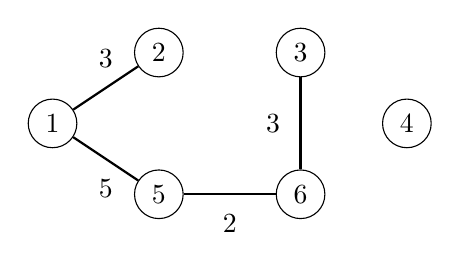
\begin{tikzpicture}[scale=0.9]
\node[draw, circle] (1) at (1.5,2) {$1$};
\node[draw, circle] (2) at (3,3) {$2$};
\node[draw, circle] (3) at (5,3) {$3$};
\node[draw, circle] (4) at (6.5,2) {$4$};
\node[draw, circle] (5) at (3,1) {$5$};
\node[draw, circle] (6) at (5,1) {$6$};

\path[draw,thick,-] (1) -- node[font=\small,label=above:3] {} (2);
%\path[draw,thick,-] (2) -- node[font=\small,label=above:5] {} (3);
%\path[draw,thick,-] (3) -- node[font=\small,label=above:9] {} (4);
\path[draw,thick,-] (1) -- node[font=\small,label=below:5] {} (5);
\path[draw,thick,-] (5) -- node[font=\small,label=below:2] {} (6);
%\path[draw,thick,-] (6) -- node[font=\small,label=below:7] {} (4);
%\path[draw,thick,-] (2) -- node[font=\small,label=left:6] {} (5);
\path[draw,thick,-] (3) -- node[font=\small,label=left:3] {} (6);
\end{tikzpicture}
\end{center}


Després d'aquests passos, la majoria de components s'han unit i hi ha
dues components a l'arbre: $\{1,2,3,5,6\}$ i $\{4\}$.

L'aresta següent de la llista és l'aresta 2--3, però no s'inclou a
l'arbre perquè els nodes 2 i 3 ja estan a la mateixa component. El
mateix passa amb l'aresta 2--5.


\begin{samepage}
Finally, the edge 4--6 will be included in the tree:

\begin{center}
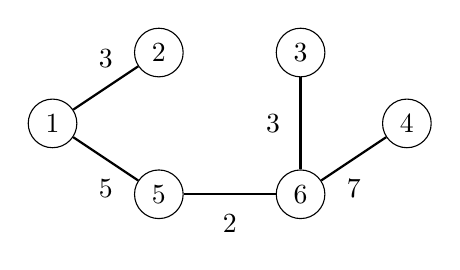
\begin{tikzpicture}[scale=0.9]
\node[draw, circle] (1) at (1.5,2) {$1$};
\node[draw, circle] (2) at (3,3) {$2$};
\node[draw, circle] (3) at (5,3) {$3$};
\node[draw, circle] (4) at (6.5,2) {$4$};
\node[draw, circle] (5) at (3,1) {$5$};
\node[draw, circle] (6) at (5,1) {$6$};

\path[draw,thick,-] (1) -- node[font=\small,label=above:3] {} (2);
%\path[draw,thick,-] (2) -- node[font=\small,label=above:5] {} (3);
%\path[draw,thick,-] (3) -- node[font=\small,label=above:9] {} (4);
\path[draw,thick,-] (1) -- node[font=\small,label=below:5] {} (5);
\path[draw,thick,-] (5) -- node[font=\small,label=below:2] {} (6);
\path[draw,thick,-] (6) -- node[font=\small,label=below:7] {} (4);
%\path[draw,thick,-] (2) -- node[font=\small,label=left:6] {} (5);
\path[draw,thick,-] (3) -- node[font=\small,label=left:3] {} (6);
\end{tikzpicture}
\end{center}
\end{samepage}


Després d'això, l'algorisme no afegeix cap aresta nova, perquè el graf
està connectat i hi ha un camí entre dos nodes qualsevol. El graf
resultant és un arbre d'expansióq mínim amb pes $2+3+3+5+7=20$.

\subsubsection{Per què funciona això?}

Es bó preguntar-se per què funciona l'algorisme de Kruskal. Com és que
aquesta estratègia greedy sempre funciona?

Vegem què passa si l'aresta de mínim pes del graf \emph{no}
s'inclogués a l'arbre d'expansió. Per exemple, suposem que l'arbre
d'expansió del graf anterior no inclou l'aresta de pes mínim
5--6. No coneixem l'estructura exacta de l'arbre d'expansió, però
sens dubte contindrà algunes arestes. Imaginem-nos un arbre com aquest:


\begin{center}
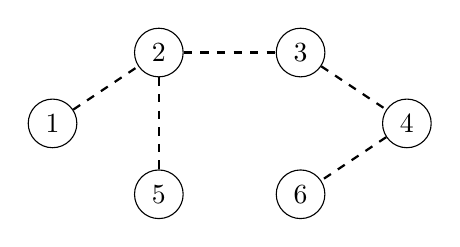
\begin{tikzpicture}[scale=0.9]
\node[draw, circle] (1) at (1.5,2) {$1$};
\node[draw, circle] (2) at (3,3) {$2$};
\node[draw, circle] (3) at (5,3) {$3$};
\node[draw, circle] (4) at (6.5,2) {$4$};
\node[draw, circle] (5) at (3,1) {$5$};
\node[draw, circle] (6) at (5,1) {$6$};

\path[draw,thick,-,dashed] (1) -- (2);
\path[draw,thick,-,dashed] (2) -- (5);
\path[draw,thick,-,dashed] (2) -- (3);
\path[draw,thick,-,dashed] (3) -- (4);
\path[draw,thick,-,dashed] (4) -- (6);
\end{tikzpicture}
\end{center}


Però no és possible que l'arbre anterior sigui un arbre d'expansió
mínim.  La raó d'això és que si afegim a aquest arbre l'aresta de pes
mínim 5--6 estem creant un cicle, i per tant podríem qualsevol altra
aresta del cicle i trobaríem un nou arbre d'expansió amb pes
\emph{menor}:


\begin{center}
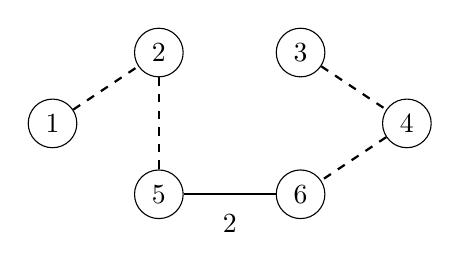
\begin{tikzpicture}[scale=0.9]
\node[draw, circle] (1) at (1.5,2) {$1$};
\node[draw, circle] (2) at (3,3) {$2$};
\node[draw, circle] (3) at (5,3) {$3$};
\node[draw, circle] (4) at (6.5,2) {$4$};
\node[draw, circle] (5) at (3,1) {$5$};
\node[draw, circle] (6) at (5,1) {$6$};

\path[draw,thick,-,dashed] (1) -- (2);
\path[draw,thick,-,dashed] (2) -- (5);
\path[draw,thick,-,dashed] (3) -- (4);
\path[draw,thick,-,dashed] (4) -- (6);
\path[draw,thick,-] (5) -- node[font=\small,label=below:2] {} (6);
\end{tikzpicture}
\end{center}


Per aquesta raó, sabem que sempre és òptim incloure qualsevol aresta
de pes mínim a l'arbre d'expansió mínim. Amb un argument similar,
podem demostrar que afegir l'aresta següent en ordre de pes també és
òptim, i així successivament. Per tant, l'algorisme de Kruskal
funciona correctament i sempre troba un arbre d'expansió mínim.

\subsubsection{Implementació}

Quan s'implementa l'algorisme de Kruskal, és convenient fer servir la
representació de llista d'arestes del graf. La primera fase de
l'algorisme ordena les arestes de la llista en temps $O(m \log m)$
temps. La segona fase de l'algorisme construeix l'arbre d'abast mínim
de la següent manera:


\begin{lstlisting}
for (...) {
  if (!same(a,b)) unite(a,b);
}
\end{lstlisting}


El bucle passa per les arestes de la llista i processa arestes de la
forma $a$--$b$. Es necessiten dues funcions: la funció \texttt{same}
determina si $a$ i $b$ estan en la mateixa component connexa, i la
funció \texttt{unite} uneix les components connexes que contenen $a$ i
$b$.

El problema és com implementar de manera eficient les funcions
\texttt{same} i \texttt{unite}. Una possibilitat és implementar la
funció \texttt{same} com a recorregut de grafs i comprovar si podem
passar del node $a$ al node $b$. Tanmateix, la complexitat temporal
d'aquesta funció seria $O(n+m)$ i l'algorisme resultant seria lent,
perquè es cridarà la funció \texttt{same} per a cada aresta del
graf.

Resoldrem el problema fent servir una estructura \emph{union-find} (o
també coneguda com \emph{merge-find-set} o \emph{MF set}) que
implementa ambdues funcions en temps $O(\log n)$. Així, la complexitat
temporal de l'algorisme de Kruskal és $O(m \log n)$ després d'ordenar
la llista de arestes.

\section{Estructura \emph{union-find}}
\label{union-find}

\index{estructura union-find}

Una \key{estructura \emph{union-find}} manté una col·lecció de
conjunts. Els conjunts són disjunts, de manera que cap element pertany
a més d'un conjunt. Aquesta estructura admet dues operacions de temps
$O(\log n)$: l'operació \texttt{unite} uneix dos conjunts, i
l'operació \texttt{find} troba el representant del conjunt que conté
un element donat\footnote{L'estructura presentada aquí va ser
introduït el 1971 per JD Hopcroft i JD Ullman \cite{hop71}. Més tard,
el 1975, R. E. Tarjan va estudiar una variant més sofisticada de
l'estructura \cite{tar75} que es discuteix en molts llibres
d'algorísmica.}.

\subsubsection{Estructura}

En una estructura \emph{union-find}, un element de cada conjunt és el
representant del conjunt, i hi ha una cadena des de qualsevol altre
element del conjunt fins al seu representant. Per exemple, suposem que
els conjunts són $\{1,4,7\}$, $\{5\}$ i $\{2,3,6,8\}$:
\begin{center}
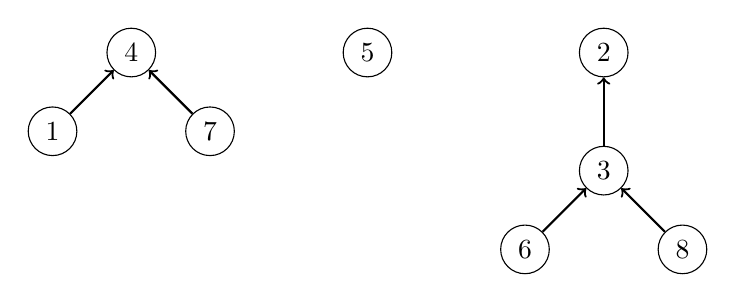
\begin{tikzpicture}
\node[draw, circle] (1) at (0,-1) {$1$};
\node[draw, circle] (2) at (7,0) {$2$};
\node[draw, circle] (3) at (7,-1.5) {$3$};
\node[draw, circle] (4) at (1,0) {$4$};
\node[draw, circle] (5) at (4,0) {$5$};
\node[draw, circle] (6) at (6,-2.5) {$6$};
\node[draw, circle] (7) at (2,-1) {$7$};
\node[draw, circle] (8) at (8,-2.5) {$8$};

\path[draw,thick,->] (1) -- (4);
\path[draw,thick,->] (7) -- (4);

\path[draw,thick,->] (3) -- (2);
\path[draw,thick,->] (6) -- (3);
\path[draw,thick,->] (8) -- (3);

\end{tikzpicture}
\end{center}
En aquest cas els representants dels conjunts són 4, 5 i 2. Podem
trobar el representant d'un element seguint la cadena que
comença en l'element donat. Per exemple, l'element 2 és el representant del conjunt
que conté l'element 6, perquè seguim la cadena $6 \rightarrow 3 \rightarrow
2$. Dos elements pertanyen al mateix conjunt exactament quan els seus
representants són els mateixos.

Podem unir dos conjunts connectant el representant d'un conjunt amb
el representant de l'altre conjunt. Per exemple, els conjunts
$\{1,4,7\}$ i $\{2,3,6,8\}$ es poden unir de la següent manera:
\begin{center}
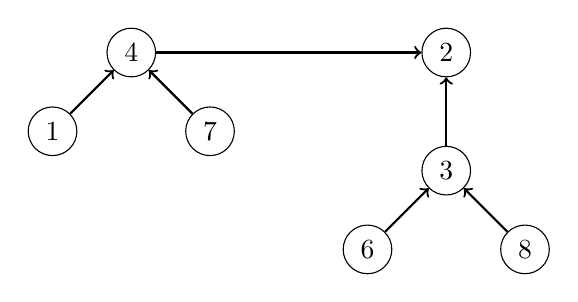
\begin{tikzpicture}
\node[draw, circle] (1) at (2,-1) {$1$};
\node[draw, circle] (2) at (7,0) {$2$};
\node[draw, circle] (3) at (7,-1.5) {$3$};
\node[draw, circle] (4) at (3,0) {$4$};
\node[draw, circle] (6) at (6,-2.5) {$6$};
\node[draw, circle] (7) at (4,-1) {$7$};
\node[draw, circle] (8) at (8,-2.5) {$8$};

\path[draw,thick,->] (1) -- (4);
\path[draw,thick,->] (7) -- (4);

\path[draw,thick,->] (3) -- (2);
\path[draw,thick,->] (6) -- (3);
\path[draw,thick,->] (8) -- (3);

\path[draw,thick,->] (4) -- (2);
\end{tikzpicture}
\end{center}


El conjunt resultant conté els elements $\{1,2,3,4,6,7,8\}$. A partir
d'aquí, l'element 2 és el representant de tot el conjunt i l'antic
representant 4 apunta a l'element 2.

L'eficiència de l'estructura d'unió-troba depèn de com s'uneixen els
conjunts. Resulta que podem seguir una estratègia senzilla: fent la
connexió des del representant del conjunt \emph{més petit} al
representant del conjunt \emph{més gran} (o, si els conjunts són de la
mateixa mida, podem fer una elecció arbitrària). Amb aquesta
estratègia, es pot veure que la longitud de qualsevol cadena és
$O(\log n)$, de manera que es pot trobar el representant de qualsevol
element de manera eficient seguint la cadena corresponent.

\subsubsection{Implementació}

L'estructura \emph{union-find} s'implementa amb vectors. En la següent
implementació, el vector \texttt{link} conté per a cada element
l'element següent de la cadena, o el propi element si és un
representant del conjunt, i el vector \texttt{size} indica per a cada
representant la mida del seu conjunt corresponent.

Inicialment, cada element pertany a un conjunt distint:
\begin{lstlisting}
for (int i = 1; i <= n; i++) link[i] = i;
for (int i = 1; i <= n; i++) size[i] = 1;
\end{lstlisting}


La funció \texttt{find} retorna el representant d'un element $x$, que
es troba seguint la cadena que comença a $x$.


\begin{lstlisting}
int find(int x) {
    while (x != link[x]) x = link[x];
    return x;
}
\end{lstlisting}


La funció \texttt{same} verifica si els elements $a$ i $b$ pertanyen
al mateix conjunt. Això es pot fer fàcilment utilitzant la funció
\texttt{find}:


\begin{lstlisting}
bool same(int a, int b) {
    return find(a) == find(b);
}
\end{lstlisting}



\begin{samepage}
The function \texttt{unite} joins the sets
that contain elements $a$ and $b$
(the elements have to be in different sets).
The function first finds the representatives
of the sets and then connects the smaller
set to the larger set.

\begin{lstlisting}
void unite(int a, int b) {
    a = find(a);
    b = find(b);
    if (size[a] < size[b]) swap(a,b);
    size[a] += size[b];
    link[b] = a;
}
\end{lstlisting}
\end{samepage}


La complexitat temporal de la funció \texttt{find} és $O(\log n)$
perquè la longitud de cada cadena és $O(\log n)$. En aquest cas, les
funcions \texttt{same} i \texttt{unite} també funcionen en temps
$O(\log n)$. La funció \texttt{unite} assegura que la longitud de cada
cadena és $O(\log n)$ perquè connecta el conjunt més petit al conjunt
més gran.

\section{Algorisme de Prim}

\index{Algorisme de Prim}

L'\key{algorisme de Prim}\footnote{L'algorisme rep el nom de
R. C. Prim que el va publicar l'any 1957 \cite{pri57}. No obstant
això, el mateix algorisme ja va ser descobert l'any 1930 per
V. Jarník.} és un mètode alternatiu per trobar un arbre d'expansió
mínim. L'algorisme afegeix primer un node arbitrari a l'arbre. Després
d'això, l'algorisme sempre tria una aresta de pes mínim que afegeix un
nou node a l'arbre. Al final, s'han afegit tots els nodes a l'arbre i
s'ha trobat un arbre d'expansió mínim.

L'algorisme de Prim s'assembla a l'algorisme de Dijkstra. La
diferència és que l'algorisme de Dijkstra sempre selecciona una aresta
la distància de la qual des del node inicial és mínima, però
l'algorisme de Prim simplement selecciona la aresta de pes mínim que
afegeix un nou node a l'arbre.

\subsubsection{Exemple}

Considerem com funciona l'algorisme de Prim en el graf següent:


\begin{center}
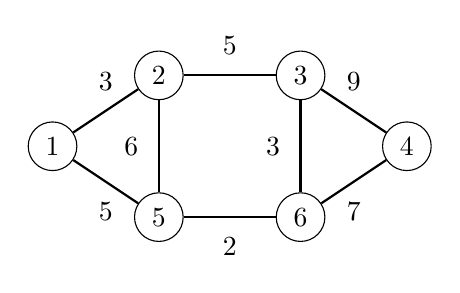
\begin{tikzpicture}[scale=0.9]
\node[draw, circle] (1) at (1.5,2) {$1$};
\node[draw, circle] (2) at (3,3) {$2$};
\node[draw, circle] (3) at (5,3) {$3$};
\node[draw, circle] (4) at (6.5,2) {$4$};
\node[draw, circle] (5) at (3,1) {$5$};
\node[draw, circle] (6) at (5,1) {$6$};
\path[draw,thick,-] (1) -- node[font=\small,label=above:3] {} (2);
\path[draw,thick,-] (2) -- node[font=\small,label=above:5] {} (3);
\path[draw,thick,-] (3) -- node[font=\small,label=above:9] {} (4);
\path[draw,thick,-] (1) -- node[font=\small,label=below:5] {} (5);
\path[draw,thick,-] (5) -- node[font=\small,label=below:2] {} (6);
\path[draw,thick,-] (6) -- node[font=\small,label=below:7] {} (4);
\path[draw,thick,-] (2) -- node[font=\small,label=left:6] {} (5);
\path[draw,thick,-] (3) -- node[font=\small,label=left:3] {} (6);

%\path[draw=red,thick,-,line width=2pt] (5) -- (6);
\end{tikzpicture}
\end{center}
Inicialment, no hi ha arestes entre els nodes:
\begin{center}
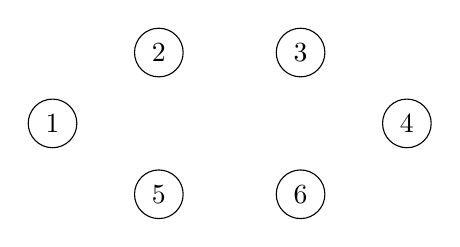
\begin{tikzpicture}[scale=0.9]
\node[draw, circle] (1) at (1.5,2) {$1$};
\node[draw, circle] (2) at (3,3) {$2$};
\node[draw, circle] (3) at (5,3) {$3$};
\node[draw, circle] (4) at (6.5,2) {$4$};
\node[draw, circle] (5) at (3,1) {$5$};
\node[draw, circle] (6) at (5,1) {$6$};
%\path[draw,thick,-] (1) -- node[font=\small,label=above:3] {} (2);
%\path[draw,thick,-] (2) -- node[font=\small,label=above:5] {} (3);
%\path[draw,thick,-] (3) -- node[font=\small,label=above:9] {} (4);
%\path[draw,thick,-] (1) -- node[font=\small,label=below:5] {} (5);
%\path[draw,thick,-] (5) -- node[font=\small,label=below:2] {} (6);
%\path[draw,thick,-] (6) -- node[font=\small,label=below:7] {} (4);
%\path[draw,thick,-] (2) -- node[font=\small,label=left:6] {} (5);
%\path[draw,thick,-] (3) -- node[font=\small,label=left:3] {} (6);
\end{tikzpicture}
\end{center}
El node inicial és un node arbitrari, així que escollim el node
1. Primer, afegim el node 2 que està connectat per una aresta de pes
3:
\begin{center}
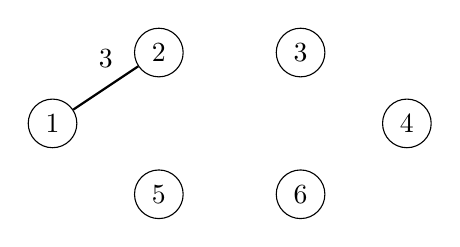
\begin{tikzpicture}[scale=0.9]
\node[draw, circle] (1) at (1.5,2) {$1$};
\node[draw, circle] (2) at (3,3) {$2$};
\node[draw, circle] (3) at (5,3) {$3$};
\node[draw, circle] (4) at (6.5,2) {$4$};
\node[draw, circle] (5) at (3,1) {$5$};
\node[draw, circle] (6) at (5,1) {$6$};
\path[draw,thick,-] (1) -- node[font=\small,label=above:3] {} (2);
%\path[draw,thick,-] (2) -- node[font=\small,label=above:5] {} (3);
%\path[draw,thick,-] (3) -- node[font=\small,label=above:9] {} (4);
%\path[draw,thick,-] (1) -- node[font=\small,label=below:5] {} (5);
%\path[draw,thick,-] (5) -- node[font=\small,label=below:2] {} (6);
%\path[draw,thick,-] (6) -- node[font=\small,label=below:7] {} (4);
%\path[draw,thick,-] (2) -- node[font=\small,label=left:6] {} (5);
%\path[draw,thick,-] (3) -- node[font=\small,label=left:3] {} (6);
\end{tikzpicture}
\end{center}


Després d'això, hi ha dos arestes amb pes 5, de manera que podem
afegir el node 3 o el node 5 a l'arbre. Afegim primer el node 3:
\begin{center}
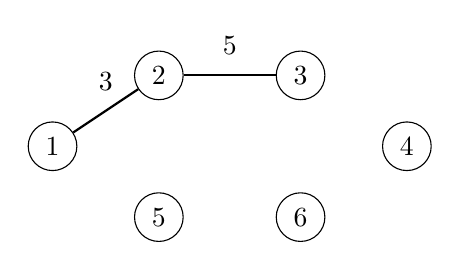
\begin{tikzpicture}[scale=0.9]
\node[draw, circle] (1) at (1.5,2) {$1$};
\node[draw, circle] (2) at (3,3) {$2$};
\node[draw, circle] (3) at (5,3) {$3$};
\node[draw, circle] (4) at (6.5,2) {$4$};
\node[draw, circle] (5) at (3,1) {$5$};
\node[draw, circle] (6) at (5,1) {$6$};
\path[draw,thick,-] (1) -- node[font=\small,label=above:3] {} (2);
\path[draw,thick,-] (2) -- node[font=\small,label=above:5] {} (3);
%\path[draw,thick,-] (3) -- node[font=\small,label=above:9] {} (4);
%\path[draw,thick,-] (1) -- node[font=\small,label=below:5] {} (5);
%\path[draw,thick,-] (5) -- node[font=\small,label=below:2] {} (6);
%\path[draw,thick,-] (6) -- node[font=\small,label=below:7] {} (4);
%\path[draw,thick,-] (2) -- node[font=\small,label=left:6] {} (5);
%\path[draw,thick,-] (3) -- node[font=\small,label=left:3] {} (6);
\end{tikzpicture}
\end{center}



\begin{samepage}
The process continues until all nodes have been included in the tree:
\begin{center}
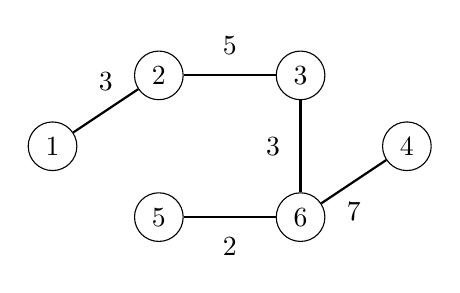
\begin{tikzpicture}[scale=0.9]
\node[draw, circle] (1) at (1.5,2) {$1$};
\node[draw, circle] (2) at (3,3) {$2$};
\node[draw, circle] (3) at (5,3) {$3$};
\node[draw, circle] (4) at (6.5,2) {$4$};
\node[draw, circle] (5) at (3,1) {$5$};
\node[draw, circle] (6) at (5,1) {$6$};
\path[draw,thick,-] (1) -- node[font=\small,label=above:3] {} (2);
\path[draw,thick,-] (2) -- node[font=\small,label=above:5] {} (3);
%\path[draw,thick,-] (3) -- node[font=\small,label=above:9] {} (4);
%\path[draw,thick,-] (1) -- node[font=\small,label=below:5] {} (5);
\path[draw,thick,-] (5) -- node[font=\small,label=below:2] {} (6);
\path[draw,thick,-] (6) -- node[font=\small,label=below:7] {} (4);
%\path[draw,thick,-] (2) -- node[font=\small,label=left:6] {} (5);
\path[draw,thick,-] (3) -- node[font=\small,label=left:3] {} (6);
\end{tikzpicture}
\end{center}
\end{samepage}


\subsubsection{Implementació}

A l'igual que l'algorisme de Dijkstra, l'algorisme de Prim
s'implementa de manera eficient amb una cua de prioritats. La cua de
prioritat ha de contenir tots els nodes que es poden connectar al
component actual mitjançant una única aresta, en ordre creixent dels
pesos de les arestes corresponents.

La complexitat temporal de l'algorisme de Prim és $O(n + m \log m)$
que és igual a la complexitat temporal de l'algorisme de Dijkstra. A
la pràctica, els algorismes de Prim i Kruskal són tots dos eficients,
i l'elecció de l'algorisme és qüestió de gustos. La majoria dels
programadors competitius fan servir l'algorisme de Kruskal.
